

\begin{figure}[H]
   \centering
   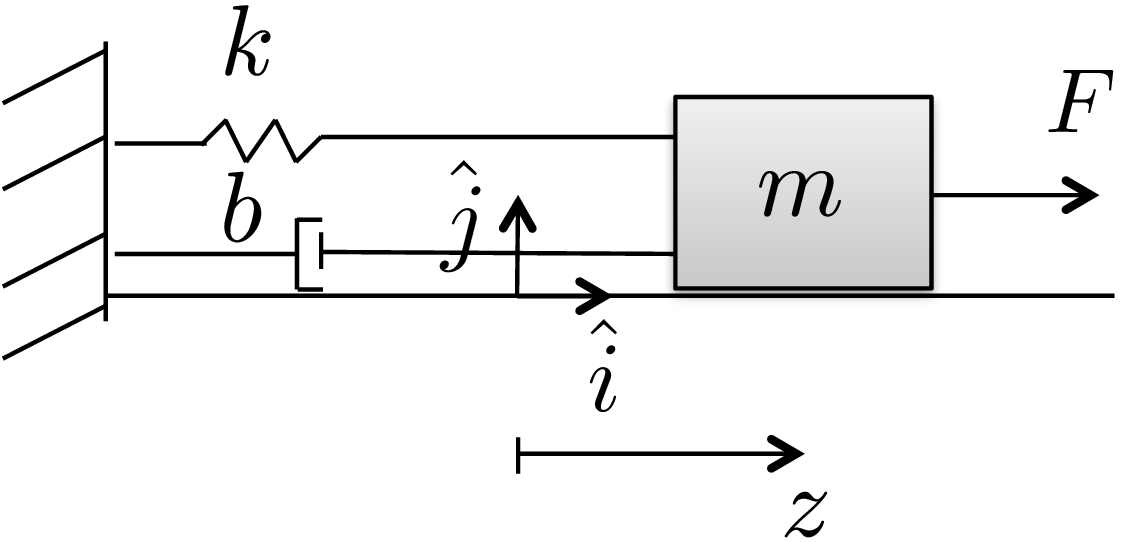
\includegraphics[width=0.5\textwidth]{./6_design_studies/figures/hw_mass_kinetic_energy} 
   \caption{Computing the kinetic energy for the mass-spring-damper.}
   \label{fig:hw_mass_kinetic_energy}
\end{figure}

The generalized coordinates for the mass spring system is the position $\mathbf{q}=z$.   The force $F$ is applied in the direction of $z$ and therefore, the generalized force is  $\boldsymbol{\tau} = F$.  There is a viscous friction force acting in the direction of $\dot{z}$ which implies that $-B\dot{\mathbf{q}} = - b\dot{z}$.

From homework \ref{hw:mass}.1, the kinetic energy can be written in terms of the generalized coordinates as
\begin{align*}
K(\mathbf{q},\dot{\mathbf{q}}) &= \frac{1}{2} m \dot{z}^2 = \frac{1}{2} m \dot{q}^2.
\end{align*}
The potential energy of the system is due to the spring force and is given by
\begin{align*}
P(\mathbf{q}) &= \frac{1}{2} k z^2 = \frac{1}{2} k q^2,
\end{align*}
where $k$ is the spring constant. 
The Lagrangian is therefore given by
\[
L(\mathbf{q},\dot{\mathbf{q}}) = K - P = \frac{1}{2} m \dot{z}^2 - \frac{1}{2} k z^2.
\]
Therefore
\begin{align*}
\frac{\partial L}{\partial\dot{\mathbf{q}}} &= m \dot{z} \\
\frac{\partial L}{\partial\mathbf{q}} &= - kz.
\end{align*}
Differentiating $\frac{\partial L}{\partial \dot{\mathbf{q}}}$ with respect to time gives
\[
\frac{d}{dt}\left(\frac{\partial L}{\partial \dot{\mathbf{q}}}\right) = m \ddot{z}.
\]
Therefore the Euler-Lagrange equation
\[
\frac{d}{dt}\left(\frac{\partial L}{\partial\dot{\mathbf{q}}} \right) - \frac{\partial L}{\partial \mathbf{q}} =  \boldsymbol{\tau} -B\dot{\mathbf{q}}
\]
gives
\[
m \ddot{z} + kz = F - b \dot{z}.
\]
